\problemname{Legendary LAN-Party}
You want to throw a LAN-Party for your $m$ best friends.
You already bought $n$ switches with $m$~LAN-ports in total.
However, only after you paid for them you realized your mistake.
You cannot connect $m$ people with those switches, since the switches themselves need to be connected.
Luckily, your switches support \emph{Power-line communication} (PLC), a technology which allows the switches to access the internet over their power cord.
Even better, you also have $n$ sockets for your power supply which support PLC.
Therefore, the only things you need to buy are the power cords for the switches.

For your party, you want to place all the switches along a line, starting with the first switch at position $1$.
The next switch would be placed right after it at position $m_1+1$, assuming the previous switch has $m_1$ ports.
You can assume that a switch with $m_i$ ports is also $m_i$ centimeter long.\looseness-1

\begin{figure}[h]
	\centering
	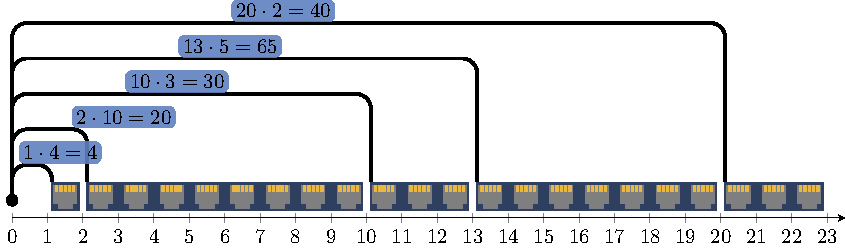
\includegraphics{sample}
	\caption{Visualization of Sample Input $1$.
		The cable length is the horizontal distance between the socket at $0$ and the start of the switch.
		The total sum of the costs is $159$.}
\end{figure}

Since all your sockets are at position $0$, you need a $1$cm cable for the first switch, a $(m_1+1)$cm cable for the second switch and so on.
Unfortunately, the costs of the cables vary for different switches.
Obviously, you do not want to pay too much for these cables.
Since the order of the switches does not matter, you want to know how much you need to pay to connect all switches?\looseness-1

\begin{Input}
	The input consists of:
	\begin{itemize}
		\item One line with two integers $n$ and $m$ $(1\leq n \leq 2\cdot10^5, 1\leq m \leq10^6)$,
			the number of network switches and the total number of ports.
		\item $n$ lines, each with two integers $c$ and $m$ $(1\leq c,m \leq
			10^6)$, the cost for one centimeter of power cable and the number of
			ports for each switch.
	\end{itemize}
\end{Input}

\begin{Output}
	Print a single integer, the minimum total cost to connect all switches.
\end{Output}
